\documentclass[12pt, a4paper]{article}
\usepackage[a4paper, left=2cm, right=2cm, top=3cm, bottom=3cm]{geometry}

\usepackage[english]{babel}
\usepackage[utf8]{inputenc}
\usepackage{fancyhdr}

\usepackage{enumitem}
\usepackage{amsmath}
\usepackage{mathtools}
\usepackage{listings}

\usepackage{tikz}
\usetikzlibrary{arrows.meta,shapes.multipart}

\pagestyle{fancy}
\fancyhf{}
\lhead{Tutorium 02 \\ Abgabegruppe 01}
\chead{Blatt 06 \\ DatKom}
\rhead{Andrés Montoya, 405409 \\ Til Mohr, 405959}

\begin{document}

\begin{center}\fcolorbox{red}{yellow}{\begin{minipage}{35em}
	Bei uns war ursprünglich noch ein Dritter in unserer Abgabegruppe eingeteilt. Wir haben ihn vor über einer Woche versucht per E-Mail zu erreichen, leider erfolglos.\\
	Nach Ablauf der Anmeldefrist zu den Abgabegruppen haben wir gesehen, dass diese Person leider unsere Abgabegruppe verlassen hat.\\
	Bisher konnten wir noch keinen Dritten für unsere Abgabegruppe finden.\\
	Uns wurde auch seit dem letzten Blatt keine weitere Person zugeteilt.
\end{minipage}}\end{center}



\section*{Aufgabe 6.1}
\begin{enumerate}[label=\alph*)]
	\item	\begin{itemize}
				\item	LAN 1: $137.226.40.0/23$
				\item	LAN 2: $137.226.42.0/25$
				\item	LAN 3: $137.226.43.0/24$
				\item	LAN 4: $137.226.42.128/27$
			\end{itemize}
	\item	Die höchste Adresse ist immer reserviert für Broadcasting und die Niedrigste repräsentiert das Netzwerk und wird nie vergeben (nach VL).\\
			
			\begin{center}\begin{tabular}{c|c|c}
				LAN & H/R & IPv4 \\
				\hline\hline
				LAN 1 & h1 & 137.226.41.254 \\
				LAN 1 & h2 & 137.226.41.253 \\
				LAN 1 & A.if1 & 137.226.40.1 \\
				\hline
				LAN 2 & h3 & 137.226.42.126 \\
				LAN 2 & A.if2 & 137.226.42.1 \\
				LAN 2 & B.if1 & 137.226.42.2 \\
				\hline
				LAN 2 & h4 & 137.226.43.254 \\
				LAN 2 & B.if2 & 137.226.43.1 \\
				\hline
				LAN 2 & h5 & 137.226.42.158 \\
				LAN 2 & B.if3 & 137.226.42.129 \\
			
			\end{tabular}\end{center}
	\item	\begin{itemize}
				\item	Paket 1: Netzwerkarte 2
				\item	Paket 2: Netzwerkarte 1
				\item	Paket 3: Netzwerkarte 8
			\end{itemize}
\end{enumerate}


\newpage


\section*{Aufgabe 6.2}
\begin{enumerate}[label=\alph*)]
	\item	\begin{center}\begin{tabular}{c|c|c|c|c|c|c|}
				Prot. & IP local & Port local & IP global & Port global & IP target & Port target \\
				\hline\hline
				\multicolumn{7}{c}{$\cdots$}\\
				\hline
				TCP & 172.16.0.16 & 6937 & 134.135.17.12 & 6938 & 212.66.4.64 & 443 \\
				TCP & 172.16.0.3 & 8532 & 134.135.17.12 & 8534 & 212.66.19.7 & 443 \\
				TCP & 172.16.0.7 & 5543 & 134.135.17.12 & 5543 & 212.66.37.12 & 443 \\
			\end{tabular}\end{center}
	\item	Port Forwarding:
			\begin{center}\begin{tabular}{c|c|c|c|c|c|c|}
				Prot. & IP local & Port local & IP global & Port global & IP target & Port target \\
				\hline\hline
				TCP & \textit{web-ip} & 80 & \textit{global-ip} & 80 & * & * \\
			\end{tabular}\end{center}
			Hierbei wird der Webserver (immer auf Port 80) local auf \textit{web-ip} gehostet und ist mit der öffentlichen IP \textit{global-ip} und Port 80 zugänglich. * steht hierfür für eine Wildcard: Es darf jeder vor Außen mit jedem Port Anfragen auf den Webserver senden: Also soll jede Anfrage auf \textit{global-ip}:80 zu unserem Webserver weitergeleitet werden.
\end{enumerate}


\newpage


\section*{Aufgabe 6.3}
\begin{itemize}
	\item	Header Länge: $20 \text{B}$
	\item	Datenlänge: $2996 \text{B} - 20 \text{B} = 2976 \text{B}$
\end{itemize}

Sei das Originalpaket: $P(\verb|TL|=2996, \verb|ID|=17, \verb|MF|=0, \verb|Offset|=744)$\\

$P$ wird an Router 1 in 2 Pakete $P_1, P_2, P_3$ geteilt mit:

\begin{itemize}
	\item	$P_1(\verb|TL|=1492, \verb|ID|=17, \verb|MF|=1, \verb|Offset|=744)$
	\item	$P_2(\verb|TL|=1492, \verb|ID|=17, \verb|MF|=1, \verb|Offset|=928)$
	\item	$P_3(\verb|TL|=52, \verb|ID|=17, \verb|MF|=0, \verb|Offset|=932)$
\end{itemize}

$P_1$, $P_2$ werden an Router 2 in Pakete $P_{11}, P_{12}, P_{13}, P_{14}, P_{21}, P_{22}, P_{23}, P_{24}$ geteilt mit:

\begin{itemize}
	\item	$P_{11}(\verb|TL|=508, \verb|ID|=17, \verb|MF|=1, \verb|Offset|=744)$
	\item	$P_{12}(\verb|TL|=508, \verb|ID|=17, \verb|MF|=1, \verb|Offset|=805)$
	\item	$P_{13}(\verb|TL|=508, \verb|ID|=17, \verb|MF|=1, \verb|Offset|=866)$
	\item	$P_{14}(\verb|TL|=28, \verb|ID|=17, \verb|MF|=1, \verb|Offset|=867)$
\\
	\item	$P_{21}(\verb|TL|=508, \verb|ID|=17, \verb|MF|=1, \verb|Offset|=928)$
	\item	$P_{22}(\verb|TL|=508, \verb|ID|=17, \verb|MF|=1, \verb|Offset|=989)$
	\item	$P_{23}(\verb|TL|=508, \verb|ID|=17, \verb|MF|=1, \verb|Offset|=1050)$
	\item	$P_{24}(\verb|TL|=28, \verb|ID|=17, \verb|MF|=1, \verb|Offset|=1051)$
\end{itemize}


\newpage


\section*{Aufgabe 6.4}
\begin{enumerate}[label=\alph*)]
	\item	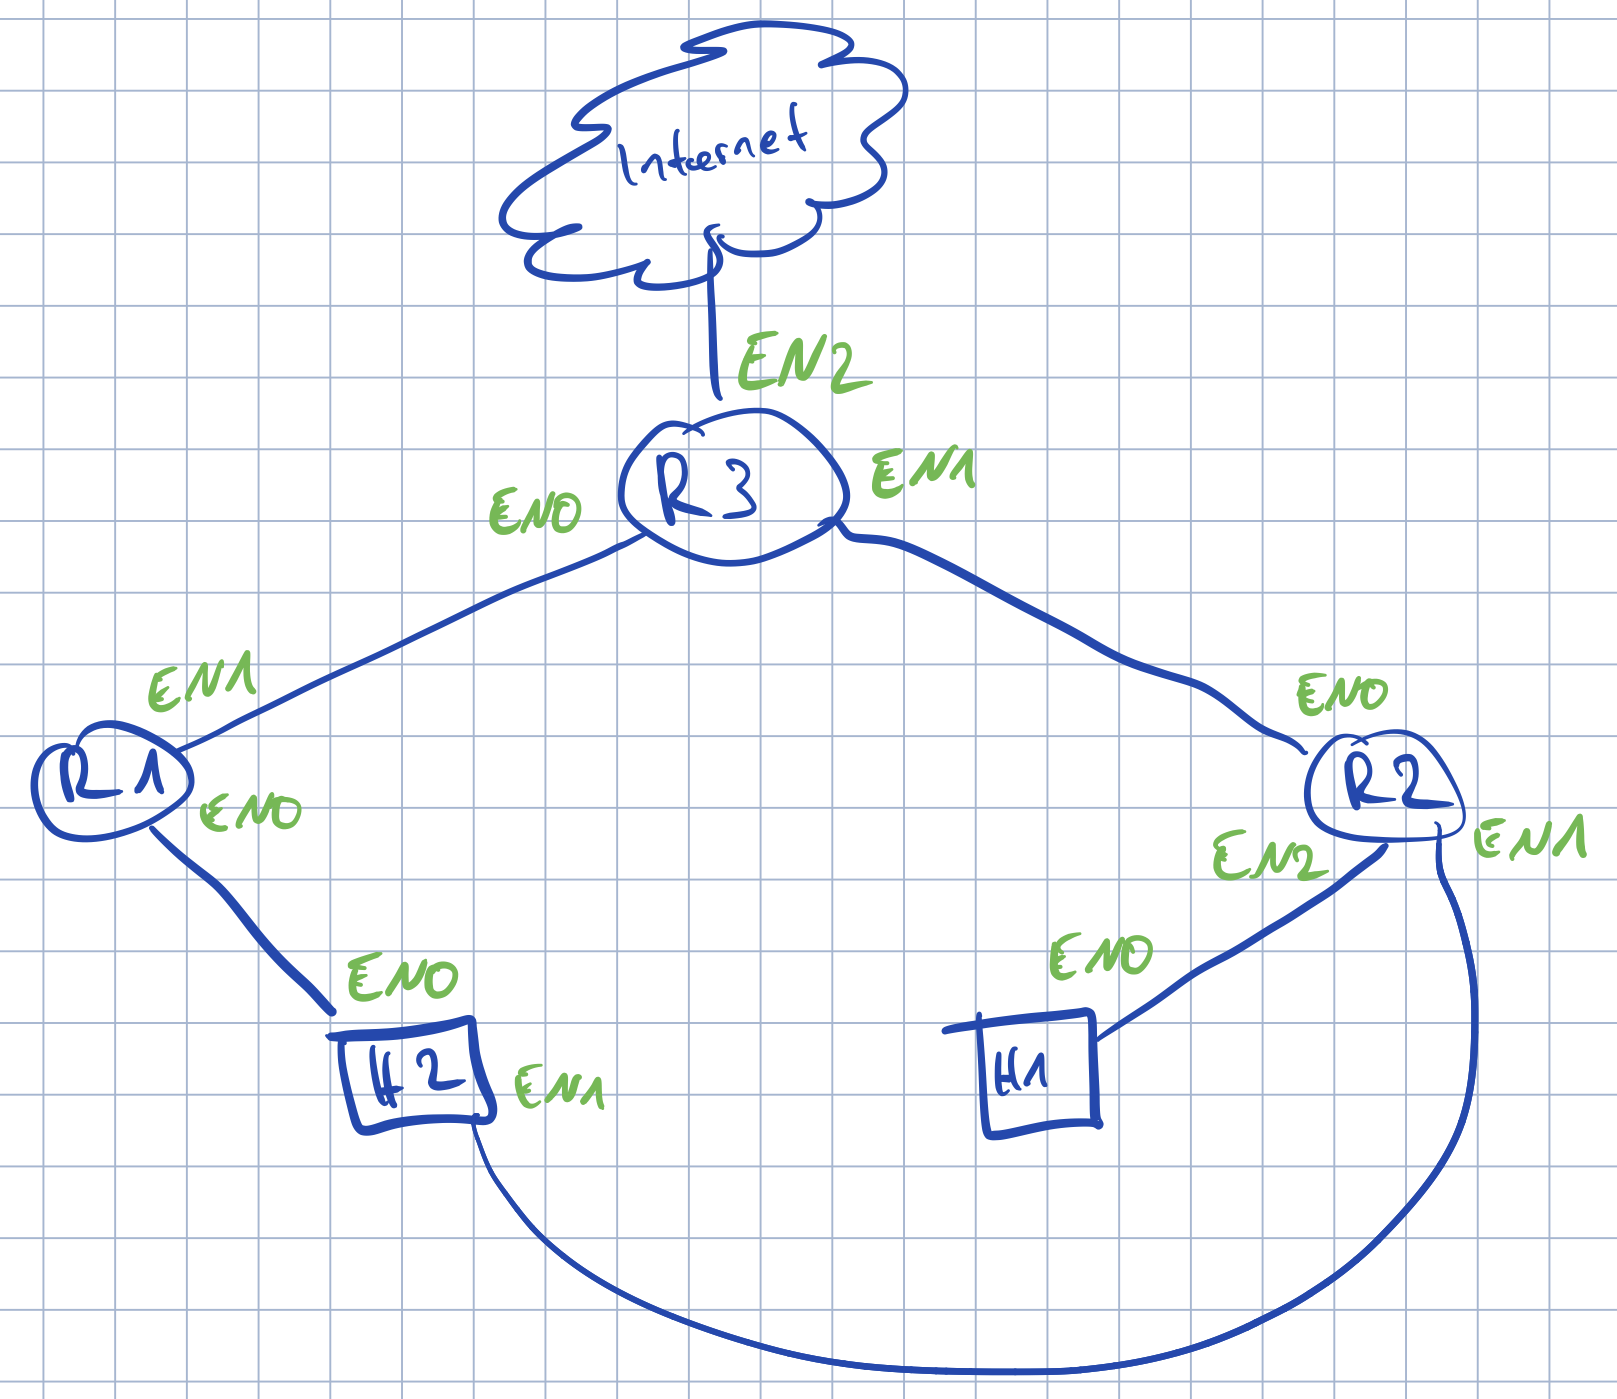
\includegraphics[scale=0.5]{6.4_a.png}
	\item	Request H2.EN0 137.226.0.243 137.226.3.234 \\
			Request H2.EN1 137.226.3.56 137.226.3.234 \\
			
			Request R1.EN1 137.226.0.1 137.226.3.234 \\
			Request R2.EN0 137.226.3.1 137.226.3.234 \\
			Request R2.EN2 137.226.3.129 137.226.3.234 \\
			
			Request R3.EN2 134.130.1.2 137.226.3.234 \\
			Response H1.EN0 137.226.3.234 R2.EN2 137.226.3.129 \\
			
			Response R2.EN2 137.226.3.129 H2.EN1 137.226.3.56 \\
			
			Data H2.EN1 H1.EN0
\end{enumerate}


\newpage


\section*{Aufgabe 6.5}
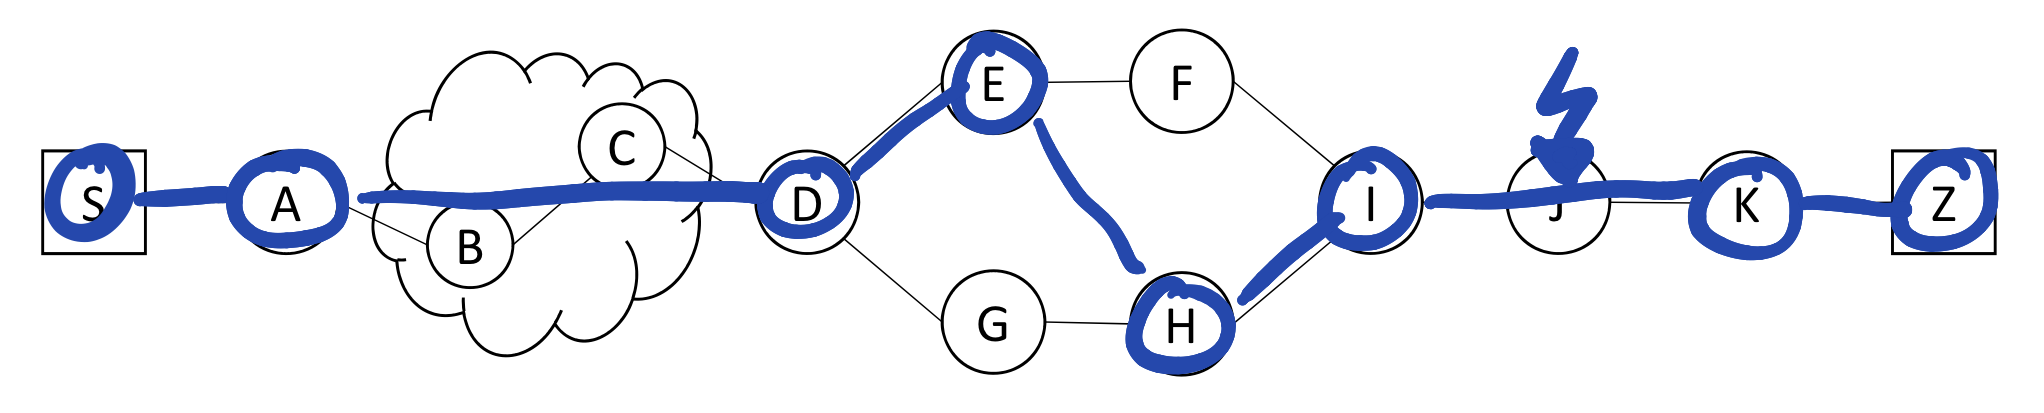
\includegraphics[scale=0.5]{6.5.png}

Die Switches $B$ und $C$ werden nicht von \verb|traceroute| ermittelt, da diese nur Layer-2-Switches sind, und somit keine keine ICMP-Nachrichten entsenden und wichtiger noch, die \verb|TTL| nicht verändern.\\
Wegen dem Loadbalancer $D$ wird erst Router $E$ als nächstes nach $D$ auf dem Pfad ermittelt, das nächste Paket geht dann jedoch wieder über $G$ zu $H$. Da darauffolgende Paket wird wieder über $E$ und dann $D$ nach $I$ gesendet. Hierdurch entsteht also eine Ungenauigkeit (da $E$ und $H$ nicht direkt verbunden sind).\\
Router $J$ entsendet zwar keine ICMP-Nachrichten, jedoch verändert er im Gegensatz zu den Switches $B$ und $C$ die \verb|TTL|. Das hierbei entstehende Problem ist, dass $S$ dieses Paket als verloren ansehen muss und somit eine \textbf{Lücke im Pfad} entsteht.

\end{document}